% Exercise ID: MAT_P4FUNCOE_4FIN_TRH_003
% Exercise ID: MAT_P4FUNCOE_4FIN_TRH_003
% Module: MÓDULO P4 - Funções | Concept: Função Inversa | Type: Teste da Reta Horizontal
% Difficulty: 2/5 (Fácil) | Type: desenvolvimento
% Points: 10 | Time: 10 min
% Tags: inversa, injetividade, teste_reta_horizontal, grafico
% Author: Professor | Date: 2025-11-18
% Status: active
% Description: Determinar quais funções são invertíveis usando teste da reta horizontal

\exercicio
Considere as funções representadas nas figuras seguintes:

\begin{figure}[H]
\centering
\begin{minipage}{0.45\textwidth}
\centering
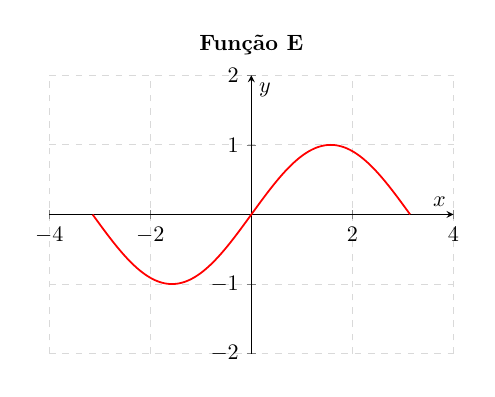
\begin{tikzpicture}[scale=0.8]
    \begin{axis}[
        axis lines = middle,
        xlabel = $x$,
        ylabel = $y$,
        xmin = -4, xmax = 4,
        ymin = -2, ymax = 2,
        grid = major,
        grid style = {dashed, gray!30},
        width = 8cm,
        height = 6cm,
        title = {Função E},
        title style = {font=\bfseries},
    ]
    \addplot[domain=-3.14:3.14, samples=200, thick, red] {sin(deg(x))};
    \end{axis}
\end{tikzpicture}
\end{minipage}
\hfill
\begin{minipage}{0.45\textwidth}
\centering
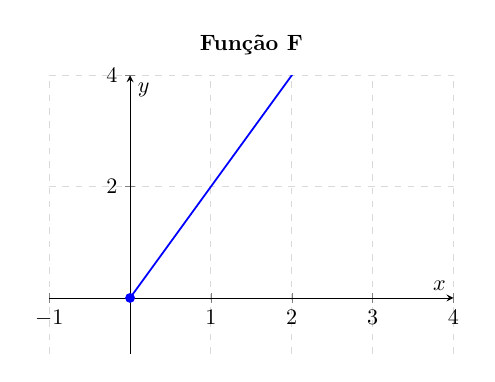
\begin{tikzpicture}[scale=0.8]
    \begin{axis}[
        axis lines = middle,
        xlabel = $x$,
        ylabel = $y$,
        xmin = -1, xmax = 4,
        ymin = -1, ymax = 4,
        grid = major,
        grid style = {dashed, gray!30},
        width = 8cm,
        height = 6cm,
        title = {Função F},
        title style = {font=\bfseries},
    ]
    \addplot[domain=0:3, thick, blue] {2*x};
    \addplot[mark=*, mark size=2pt, blue] coordinates {(0,0)};
    \addplot[mark=*, mark size=2pt, blue] coordinates {(3,6)};
    \end{axis}
\end{tikzpicture}
\end{minipage}
\end{figure}



Quais das duas funções são invertíveis (isto é, cuja inversa também é uma função)? Justifique usando o teste da reta horizontal.

\vspace{3cm}
